\documentclass[11pt,a4paper]{article}

\usepackage[utf8]{inputenc}
\usepackage[T1]{fontenc}
\usepackage[margin=25mm]{geometry}
\usepackage{booktabs}
\usepackage{tabularx}
\usepackage{array}
\usepackage{enumitem}
\usepackage{xcolor}
\usepackage{listings}
\usepackage{tikz}
\usetikzlibrary{arrows.meta,positioning,shapes.geometric}
\usepackage[hidelinks]{hyperref}

\lstset{
    language=C++,
    basicstyle=\ttfamily\small,
    columns=fullflexible,
    keepspaces=true,
    frame=single,
    breaklines=true,
    showstringspaces=false
}
\setlist{nosep}
\setlength{\parskip}{0.45em}
\setlength{\parindent}{0pt}

\title{\textbf{RouteCraft}\\Multi-Depot Vehicle Routing Studio}
\author{
    AlgoSmiths\\
    106125071 -- Meesala Hariteja\\
    106125069 -- Mayank Gupta\\
    106125067 -- Matta Jay Paul
}
\date{CSLR31 Data Structures Laboratory Project}

\begin{document}
\maketitle

\begin{abstract}
RouteCraft is a visual route-planning application for the capacitated multi-depot vehicle routing problem.\\
The problem is to serve customer demands from available depots while respecting vehicle capacity and fleet limits.\\
Poorly planned delivery trips can increase distance, time, and operating cost for local delivery fleets.\\
The project explores how data structures and algorithms can support this practical logistics problem.\\
Existing fleet-planning products provide routing capabilities, but may be costly or complex for a classroom demonstration.\\
Our objective is to build an approachable desktop prototype that makes route construction and its results visible.\\
Users can create depots and customers, assign demands, and choose a vehicle count and capacity.\\
The application can import OpenStreetMap XML roads and calculate weighted shortest paths through the road graph.\\
Clarke--Wright savings and nearest-neighbor methods construct capacity-aware routes for multiple depots.\\
Two-opt and three-opt-lite local search attempt to improve the constructed routes.\\
The Java Swing interface communicates with a modular C++ DSA engine through the Java Native Interface.\\
Future work includes stronger VRP heuristics, time windows, traffic-aware estimates, and broader automated testing.
\end{abstract}

\section{Step 1 -- Problem identification and idea}

\subsection{Problem statement and motivation}
The capacitated multi-depot vehicle routing problem (MDVRP) asks how a fleet
based at multiple depots should visit a set of customers with known demands.
Each route begins and ends at a depot, each vehicle has a capacity limit, and
the available fleet is bounded. A poor route plan can waste travel distance
and time. RouteCraft provides an educational, interactive way to model this
problem and observe the effect of route construction and local-search
algorithms.

The prototype is aligned with Sustainable Development Goal 11 (Sustainable
Cities and Communities) through its exploration of more efficient urban
delivery planning. It is not a production logistics service and does not claim
measured environmental or operational savings. Its objective is to demonstrate
how graph algorithms, route heuristics, and capacity constraints can be
combined in a usable application.

\subsection{Objectives and salient features}
\begin{itemize}
    \item Model multiple depots, customers, customer demand, vehicle count,
          and per-vehicle capacity.
    \item Construct routes using Clarke--Wright savings or nearest neighbor,
          then apply two-opt and three-opt-lite improvements.
    \item Import a compact OpenStreetMap XML road extract and route on its
          directed road graph; use straight-line distances when no road graph
          is loaded.
    \item Compare distance, estimated time, estimated cost, and a weighted
          objective score.
    \item Display route manifests and animate dispatch; export route details
          as CSV.
\end{itemize}

\subsection{Existing products and project scope}
Commercial and open mapping products provide road directions and fleet
features. RouteCraft is intentionally narrower: it is a self-contained
classroom prototype focused on demonstrating DSA concepts and exposing the
route plan. The routing procedures are heuristics and do not guarantee a
global optimum. Speeds and costs are estimates, not live traffic or quotes. A route without
an imported road graph has no geographic scale, so its distance is reported
in map units rather than kilometres.

\section{Step 2 -- Product design and module workflow}

\subsection{Flowchart}
The diagram below shows both the road-network and coordinate fallback paths.
The editable TikZ source is in \texttt{Document/RouteCraft\_Flowchart.tex};
it can be imported into the Overleaf report project.

\begin{center}
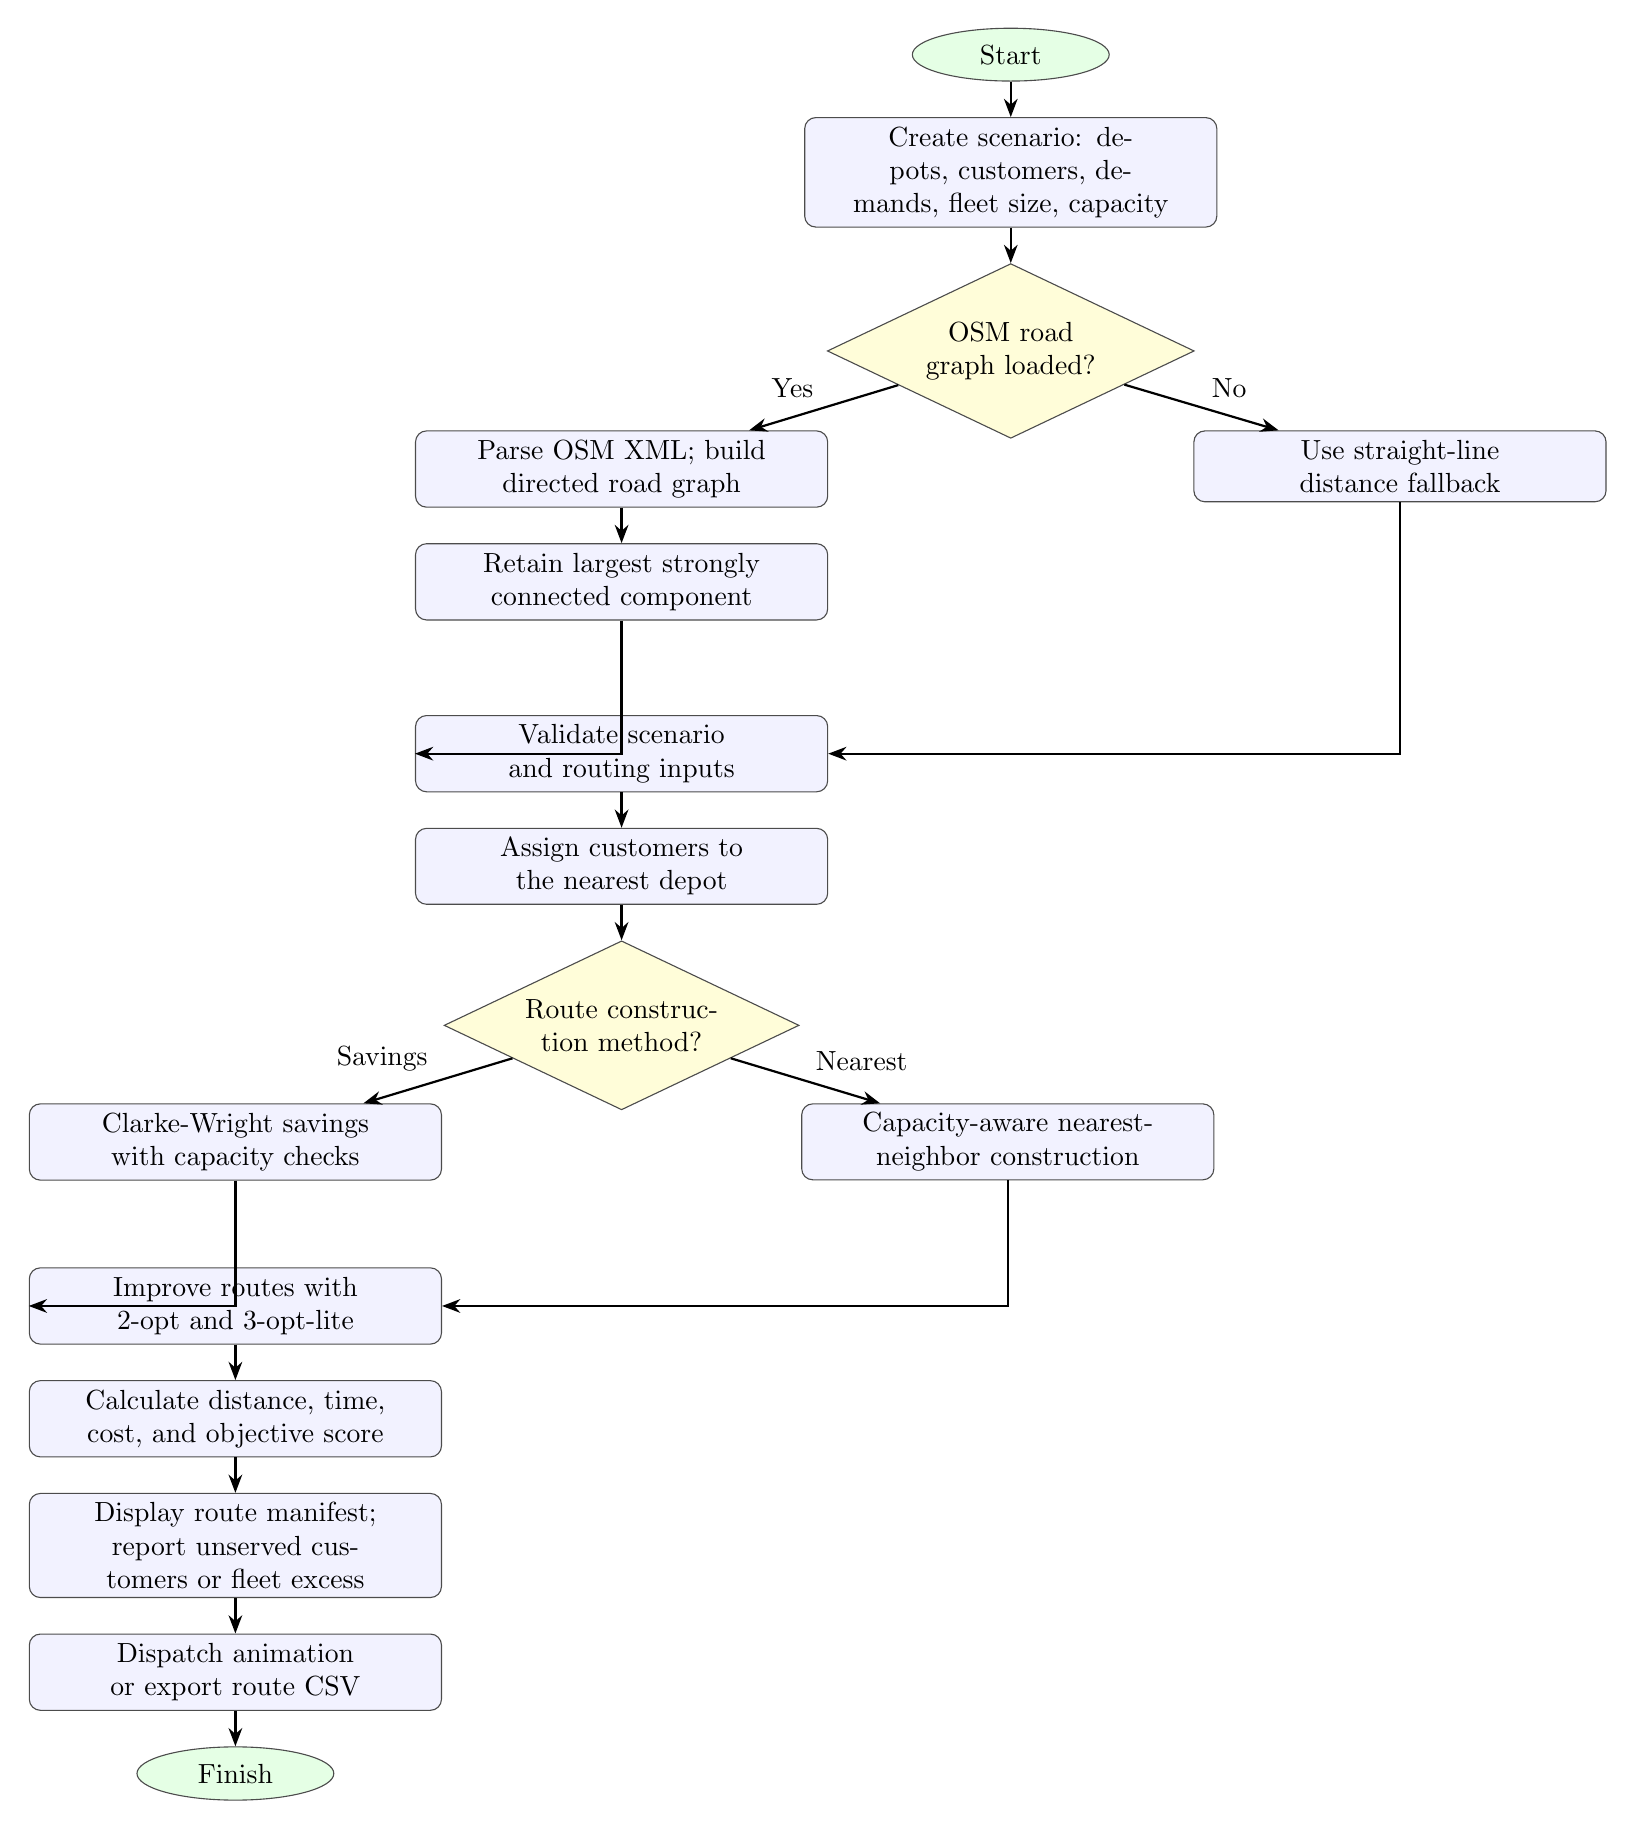
\begin{tikzpicture}[
    node distance=0.45cm and 1.15cm,
    process/.style={
        rectangle,
        rounded corners,
        draw=black!70,
        fill=blue!5,
        align=center,
        text width=5.0cm,
        minimum height=0.75cm
    },
    decision/.style={
        diamond,
        aspect=2.1,
        draw=black!70,
        fill=yellow!15,
        align=center,
        text width=2.9cm,
        inner sep=1pt
    },
    startstop/.style={
        ellipse,
        draw=black!70,
        fill=green!10,
        align=center,
        minimum width=2.5cm,
        minimum height=0.65cm
    },
    arrow/.style={-Stealth, thick}
]
\node[startstop] (start) {Start};
\node[process, below=of start] (scenario) {Create scenario: depots, customers, demands, fleet size, capacity};
\node[decision, below=of scenario] (osmchoice) {OSM road graph loaded?};
\node[process, below left=of osmchoice] (osm) {Parse OSM XML; build directed road graph};
\node[process, below=of osm] (scc) {Retain largest strongly connected component};
\node[process, below right=of osmchoice] (fallback) {Use straight-line distance fallback};
\node[process, below=1.2cm of scc] (validate) {Validate scenario and routing inputs};
\node[process, below=of validate] (assign) {Assign customers to the nearest depot};
\node[decision, below=of assign] (method) {Route construction method?};
\node[process, below left=of method] (savings) {Clarke-Wright savings with capacity checks};
\node[process, below right=of method] (nearest) {Capacity-aware nearest-neighbor construction};
\node[process, below=1.1cm of savings] (improve) {Improve routes with 2-opt and 3-opt-lite};
\node[process, below=of improve] (score) {Calculate distance, time, cost, and objective score};
\node[process, below=of score] (display) {Display route manifest; report unserved customers or fleet excess};
\node[process, below=of display] (actions) {Dispatch animation or export route CSV};
\node[startstop, below=of actions] (finish) {Finish};

\draw[arrow] (start) -- (scenario);
\draw[arrow] (scenario) -- (osmchoice);
\draw[arrow] (osmchoice) -- node[above left]{Yes} (osm);
\draw[arrow] (osm) -- (scc);
\draw[arrow] (osmchoice) -- node[above right]{No} (fallback);
\draw[arrow] (scc.south) |- (validate.west);
\draw[arrow] (fallback.south) |- (validate.east);
\draw[arrow] (validate) -- (assign);
\draw[arrow] (assign) -- (method);
\draw[arrow] (method) -- node[above left]{Savings} (savings);
\draw[arrow] (method) -- node[above right]{Nearest} (nearest);
\draw[arrow] (savings.south) |- (improve.west);
\draw[arrow] (nearest.south) |- (improve.east);
\draw[arrow] (improve) -- (score);
\draw[arrow] (score) -- (display);
\draw[arrow] (display) -- (actions);
\draw[arrow] (actions) -- (finish);
\end{tikzpicture}

\end{center}

\subsection{Modules and data flow}
\textbf{User interface and scenario module.}
\texttt{RouteCraftVRP.java} implements the Java Swing workspace. It
maintains depot and customer records, accepts demand and fleet settings,
renders the map and route manifests, supports scenario undo/redo, and exports
CSV. The application reports the number of served customers and routes so an
infeasible fleet or capacity setting is visible.

\textbf{OSM import and road graph.}
The Java importer reads OSM XML nodes, ways, and tags; rejects unsafe XML
external-entity processing; filters routable highway types; and creates
directed edges to reflect one-way roads. It estimates edge distance, time,
and cost. Road coordinates are normalized for display. When a road graph is
provided, the C++ engine retains its largest strongly connected component.
The application otherwise falls back to direct coordinate distance.

\textbf{C++ model and optimization module.}
\texttt{include/RouteObjects.h} and
\texttt{source/RouteObjects.cpp} define nodes, road edges, routes, and legs.
\texttt{include/RouteOptimizer.h} declares the optimizer, and
\texttt{source/RouteOptimizer.cpp} defines its algorithms. Customer groups
are assigned to their nearest depot. Nearest-neighbor construction repeatedly
chooses a feasible unserved customer. Clarke--Wright savings merges route
ends when the capacity limit is respected \cite{clarke1964}. Two-opt and
three-opt-lite reverse route segments when the weighted objective improves.

For real road legs, Dijkstra's algorithm searches the directed graph using a
weighted combination of distance, estimated time, and cost
\cite{dijkstra1959}. Kosaraju's two-pass graph traversal finds strongly
connected components. Nodes and routes are owned by \texttt{std::shared\_ptr};
road-edge links use \texttt{std::weak\_ptr} to avoid ownership cycles.

\textbf{JNI adapter.}
\texttt{RouteOptimizerBridge.java} converts Java model data to native
arrays and converts results back to Java routes. The C++ exports in
\texttt{source/RouteOptimizerJni.cpp} validate array shapes, manage a native
engine handle, transfer the road graph, and expose optimization and metric
operations. The bridge is a data adapter; routing algorithms remain in C++.

\textbf{Build and test modules.}
\texttt{source/RouteCraftDsaTests.cpp} is the C++ test runner. The Java-side
integration runner is \texttt{RouteOptimizerBridgeTest.java}. The root
\texttt{Makefile} builds the C++ objects, test executable, JNI library, and
Java classes. \texttt{run.bat} builds and launches the desktop application on
Windows.

\section{Step 3 -- Coding and modular organization}

The project separates declarations from definitions as required:
\texttt{include/} contains C++ declarations; \texttt{source/} contains only
the C++ model, optimizer, JNI implementation, and native test runner. The
Java Swing interface, JNI adapter, and bridge test remain at the project
root. \texttt{object/} contains compiled C++ object files. The native and
Java interface are compiled with a matching 64-bit toolchain. Build
instructions and the user manual are maintained in \texttt{README.md} and
\texttt{Document/User\_Manual.md}.

The following excerpt illustrates the two-opt improvement condition used by
the C++ optimizer:

\begin{lstlisting}
if (distance(b, l) + distance(f, a) + TWO_OPT_EPSILON
        < distance(b, f) + distance(l, a)) {
    std::reverse(route.stops.begin() + i, route.stops.begin() + k + 1);
    imp = true;
}
\end{lstlisting}

\section{Step 4 -- Test cases and test data}

The test data is deterministic and generated in the test programs. Coordinate
tests use a depot at $(0,0)$ and a customer at $(3,4)$; the default synthetic
model produces a round trip of 10 map units, 20 estimated minutes, and 120
estimated cost units. Capacity tests use two depots and three customers with
demands 2, 3, and 1, using two vehicles of capacity 5. Graph tests use two
mutually reachable nodes and one isolated node.

\begin{table}[h]
\centering
\small
\begin{tabularx}{\textwidth}{@{}p{0.20\textwidth}X p{0.13\textwidth}@{}}
\toprule
\textbf{Test} & \textbf{Expected result} & \textbf{Result}\\
\midrule
Round-trip metrics and geographic distance
    & Distance, time, cost, weighted score, and equatorial degree distance
      match their expected values.
    & PASS\\
Capacity and customer coverage (nearest neighbor)
    & All feasible customers appear once; every route load is at most 5; no
      more than two routes are returned.
    & PASS\\
Capacity and customer coverage (savings)
    & The same coverage and capacity conditions hold for the savings method.
    & PASS\\
Strongly connected component filtering
    & The two-node mutually reachable component is retained; the isolated
      node and external edges are removed.
    & PASS\\
Invalid optimizer input
    & Customers without a depot produce an explicit input error.
    & PASS\\
JNI graph and optimization integration
    & Java graph transfer, SCC filtering, nearest-node lookup, road-leg
      metrics, route metrics, and route/customer mapping work through JNI.
    & PASS\\
\bottomrule
\end{tabularx}
\caption{Automated test results from \texttt{mingw32-make test}.}
\end{table}

The automated checks do not replace a live UI demonstration. Before final
submission, the team should also demonstrate adding a scenario, importing a
small valid \texttt{.osm} extract, optimizing, dispatching, and exporting CSV.

\section{Step 5 -- Contributions, takeaways, and future scope}

\subsection{Individual contributions}
The team has not yet verified a person-by-person task breakdown. The
following entries are intentionally marked pending; the team must replace
them with factual work completed by each member before submission.

\begin{table}[h]
\centering
\begin{tabularx}{\textwidth}{@{}p{0.19\textwidth}p{0.30\textwidth}X@{}}
\toprule
\textbf{Registration number} & \textbf{Member} & \textbf{Verified contribution}\\
\midrule
106125071 & Meesala Hariteja & Pending team verification.\\
106125069 & Mayank Gupta & Pending team verification.\\
106125067 & Matta Jay Paul & Pending team verification.\\
\bottomrule
\end{tabularx}
\end{table}

\subsection{Key takeaways}
\begin{enumerate}
    \item A graph representation makes real road networks available to route
          algorithms while keeping coordinate fallback possible.
    \item Capacity and fleet constraints must be checked during construction
          and communicated when some customers remain unserved.
    \item Local search improves heuristic routes but cannot establish global
          optimality for the general routing problem.
    \item JNI allows a Java interface and a C++ DSA engine to share one
          application while requiring careful validation of native data
          boundaries.
    \item Automated tests are valuable for algorithmic invariants and bridge
          correctness, but UI workflows still need human demonstration.
\end{enumerate}

\subsection{Future scope}
Possible extensions include time windows, heterogeneous vehicles, vehicle
start/end constraints, traffic-aware travel estimates, alternative
metaheuristics, richer infeasibility reports, persisted scenarios, and
performance tests on larger OSM extracts.

\subsection{Acknowledgements}
None specified by the team.

\section*{References}
\begin{thebibliography}{9}
\bibitem{clarke1964}
G. Clarke and J. W. Wright, ``Scheduling of Vehicles from a Central Depot to
a Number of Delivery Points,'' \textit{Operations Research}, vol. 12, no. 4,
pp. 568--581, 1964. doi: \href{https://doi.org/10.1287/opre.12.4.568}
{10.1287/opre.12.4.568}.

\bibitem{dijkstra1959}
E. W. Dijkstra, ``A Note on Two Problems in Connexion with Graphs,''
\textit{Numerische Mathematik}, vol. 1, pp. 269--271, 1959. doi:
\href{https://doi.org/10.1007/BF01386390}{10.1007/BF01386390}.

\bibitem{osm}
OpenStreetMap contributors, ``Copyright and License.''
\url{https://www.openstreetmap.org/copyright} (accessed 27 October 2026).

\bibitem{osmtiles}
OpenStreetMap Foundation, ``Tile Usage Policy.''
\url{https://operations.osmfoundation.org/policies/tiles/}
(accessed 27 October 2026).

\bibitem{jni}
Oracle, ``Java Native Interface (JNI) Specification.''
\url{https://docs.oracle.com/en/java/javase/17/docs/specs/jni/}.

\bibitem{sdg}
United Nations Educational, Scientific and Cultural Organization,
``Sustainable Development Goals.''
\url{https://www.unesco.org/en/sdgs}.
\end{thebibliography}

\end{document}
